  \documentclass[twoside=false, %  doppelseitiger Druck
    DIV=15,% DIV Faktor für Satzspiegelberechnung, sie Doku zu KOMA Script
    BCOR=15mm, % Bindekorrektur
    chapterprefix=false,
    headinclude=true,
    footinclude=false,
    pagesize,%         write pagesize to DVI or PDF
    fontsize=11pt,%             use this font size
    paper=a4,%          use ISO A4
    bibliography=totoc,%         write bibliography-chapter to table of contents
    index=totoc,%         write index-chapter to table of contents
    cleardoublepage=plain,% \cleardoublepage generates pages with pagestyle empty
     headings=big,%       A4/B5
    listof=flat,%        improved list of tables
    numbers=noenddot
  ]{scrbook}

\usepackage[utf8]{inputenc}
\usepackage{makeidx}
\usepackage{amsfonts}
\usepackage[slantedGreek,sc]{mathpazo}  % Schriftart Palatino
% \usepackage{lmodern}    % statt mathpazo, falls CM Fonts verwendet werden sollen
%\usepackage{mathptmx}    % statt mathpazo, falls Times  verwendet werden soll
\usepackage[scaled=.95]{helvet}
\usepackage{courier}
\usepackage[T1]{fontenc}
\usepackage{textcomp}
\usepackage{amsmath}            % standard math notation (vectors/sets/...)
\usepackage{bm}        % standard math notation (fonts)
\usepackage{fixmath}        % standard math notation (fonts)
\usepackage{graphicx}
\usepackage[facing=yes]{floatrow}       % mehrere Gleitobjekte nebeneinander/caption neben Bild/Tabelle
\usepackage[labelfont=bf,sf,font=small,labelsep=space,format=plain]{caption}
\usepackage{subcaption}
\usepackage{scrlayer-scrpage}
% \usepackage{pstool}  % einbinden falls psfrag verwendet werden soll
\usepackage{epstopdf}
\usepackage[ngerman]{babel}
\usepackage{ellipsis}  % Korrigiert den Weißraum um Auslassungspunkte
\usepackage{microtype}  % optischer Randausgleich etc.

\usepackage{xcolor}         % z.B. für schattierte Boxen
\usepackage{framed}			% shaded Umgebung
\definecolor{shadecolor}{gray}{.85}%

% Links im PDF
\usepackage[colorlinks=false,
            pdfborder={0 0 0},
            breaklinks=true]
            {hyperref}


%\typearea[current]{calc}


% Einstellungen für Bild-/Tabellenbeschriftung neben dem Bild
\floatsetup[figure]{capbesideposition={inside,top}}
\floatsetup[table]{capbesideposition={inside,top},style=plaintop}
\renewfloatcommand{fcapside}{figure}[\capbeside][\FBwidth]
\newfloatcommand{tcapside}{table}[\capbeside][\FBwidth]


\selectlanguage{ngerman}


\deffootnote{1em}{1em}{%
 \makebox[1em][l]{\thefootnotemark}}

\makeindex

\newcommand{\real}{\mathord{\mathrm{I\!R}}}

\begin{document}
\selectlanguage{ngerman}
\def\figdir{figures}
\def\tabledir{tables}

\frontmatter

\pagestyle{scrplain}
\pagestyle{empty}

\begin{titlepage}

\sffamily

\raggedleft

\vspace*{-2cm}


\includegraphics{\figdir/logo-th-rosenheim-2019_master_quer_2c.eps}

\vfill

\centering
\LARGE
% \vspace*{\fill}
%-----------
Fakultät für Informatik  \vspace{0.5cm}\\
\Large
Studiengang Software- und Systems-Engineering

\vspace{2cm}

\LARGE

Erkennung von Design Patterns in Quellcode durch Machine Learning

\vspace{2cm}

\Large
Master Thesis

\vspace{1.5cm}


\Large
von

\vspace{0.5cm}

%\vspace*{\fill}

\LARGE
Mehmet Aslan \vspace{1cm}

\vspace{1cm}

\flushleft
 \Large
\vspace*{\fill}

%-----------
\begin{tabbing}
Datum der Abgabe: \= 18.02.2024 \kill
Datum der Abgabe: \> 18.02.2024 \\
Erstprüfer: \> Prof.\ Dr.\ Marcel Tilly\\
Zweitprüfer: \> Prof.\ Dr.\ Kai Höfig
\end{tabbing}
%-----------

\end{titlepage}

\cleardoubleemptypage

{
\large
\thispagestyle{empty}
\vspace*{\fill}

\noindent
\textsc{Eigenständigkeitserklärung / Declaration of Originality}

\medskip

\noindent
Hiermit bestätige ich, dass ich die vorliegende Arbeit selbständig verfasst und keine anderen als die angegebenen Hilfsmittel benutzt habe. Die Stellen der Arbeit, die dem Wortlaut oder dem Sinn nach anderen Werken (dazu zählen auch Internetquellen) entnommen sind, wurden unter Angabe der Quelle kenntlich gemacht.

\medskip

\textit{I declare that I have authored this thesis independently, that I have not used other than the declared sources / resources, and that I have explicitly marked all material which has been quoted either literally or by content from the used sources.}

\bigskip

\noindent
München, den 18.02.2024

\vspace*{2cm}

\noindent
Mehmet Aslan
}

%%% Local Variables: 
%%% mode: latex
%%% TeX-master: "d"
%%% End: 

\cleardoubleemptypage
\chapter*{Kurzfassung}
\thispagestyle{empty}

Design Patterns oder Entwurfsmuster sind in der Software-Entwicklung gängige Lösungsansätze für wiederkehrende Probleme.
Von Software-Entwicklern werden diese eingesetzt, um Probleme in der Implementierung oder in der Software-Architektur zu lösen, deren Lösungsweg bereits bekannt sind und für die jeweilige Situation abgeändert werden. Die wohl bekanntesten Design Patterns sind die 23 Entwurfsmuster nach Gamma et al.
Im weiteren Verlauf der Software-Entwicklung sind die eingesetzten Entwurfsmuster aufgrund iterativer Änderungen und steigender Komplexität im Quellcode nicht mehr einfach wiederzufinden.
Deswegen liegt der Fokus dieser Masterthesis auf der Etablierung eines Prozesses, welcher mit Machine Learning in der Lage ist, Design Pattern im Quellcode zu erkennen.

Das Ziel dieser Arbeit ist es, die Entwurfsmuster Singleton, Observer, Command und Adapter zu identifizieren. Im Kontext dieser Arbeit werden diese als Strukturen definiert, die in Summe von Rollen dargestellt werden.
Jedes dieser Rollen übernimmt im Kontext des jeweiligen Design Patterns unterschiedliche Aufgaben und Verantwortungen.
Dazu wird ein Klassifizierer trainiert, welches Rollen innerhalb dieser Entwurfsmuster durch Code-Metriken erkennt.
Anhand der Klassifikation der Rollen wird im finalen Schritt ein Übereinstimmungswert berechnet, der angibt, mit welcher Zuversicht es sich hierbei um das jeweilige Entwurfsmuster handelt.
Zum Schluss wird die Klassifikationsleistung der hier vorgestellten Methode anhand der Metriken \textit{Precision}, \textit{Recall} und \textit{f1} evaluiert. 

\bigskip

\noindent
Schlagworte: Software-Entwicklung, Machine Learning, Design Patterns 


\cleardoubleemptypage

\pagestyle{scrplain}
\pagenumbering{roman}
% ---------------------------------------------------
% D-TOC.TEX zur Verwendung mit TEXPART
% (an eigene Gegebenheiten anzupassen)
% ---------------------------------------------------
%
\tableofcontents
\clearpage
\listoffigures
\clearpage
\listoftables
\cleardoublepage


\pagestyle{scrheadings}


\addtokomafont{caption}{\small}

\mainmatter

\chapter{Motivation}
\section{Einführung in Design Patterns}

Entwurfsmuster oder auf Englisch `Design Patterns' sind bewährte Lösungsansätze für wiederkehrende Probleme, die bei der Konzeption der Software-Architektur oder während der Implementierung der Software
eingesetzt werden kann. Dabei dienen diese Entwurfsmuster als eine Art Blaupause, die es Software-Entwicklern ermöglicht, erprobte Lösungsstrategien für häufig auftretende Probleme in der Software-Entwicklung anzuwenden.
Durch den Einsatz von etablierten Entwurfsmustern können Software-Entwickler für die Software bei korrekter Anwendung unter anderem erhöhte Wartbarkeit, Wiederverwendbarkeit von Komponenten, Verständlichkeit und Skalierbarkeit ermöglichen das wiederum in qualitativ besserer Software resultiert.
Dabei sollte beachtet werden, dass Design Patterns als Vorlage zu betrachten sind. Je nach Einsatzgebiet muss die Anwendung des Entwurfsmusters evaluiert und für den konkreten Fall individualisiert werden.
Deshalb existiert keine universelle anwendbare Iteration eines Design Patterns, die unabhängig von Anwendungskontext eingesetzt werden kann. Dies resultiert in variierenden Anwendung von Entwurfsmustern abhängig von jeweiligem Einsatzgebiet.
Im weiteren Entwicklungszyklus der Software werden durch neue oder geänderte Anforderungen bereits eingesetzte Implementierungen von Entwurfsmustern modifiziert, entfernt oder neue werden hinzugefügt.
Währenddessen besteht die Gelegenheit, dass durch mangelnder Dokumentation oder anderer Gründe die Entscheidungen, weshalb Entwurfsmuster so eingesetzt sind wie es eingesetzt worden, verloren gehen.
Dadurch besteht die Gefahr, dass angewendete Design Patterns im weiteren Verlauf derer Entwicklung nicht mehr wiederzuerkennen sind. Aus diesem Grund ist die Etablierung eines Prozesses von Vorteil, das in der Lage ist,
Implementierungen von Entwurfsmustern aus einem Software-System zu extrahieren und dieses konkret benennen. Vor allem der Einsatz von Maschine Learning für die Klasszifierung ist hier vorteilhaft, wodurch das Potenzial besteht, vorher nicht gesehene Implementierung von Design Patterns zu erkennen.
Durch solch einen Prozess können durch die Erkennung von eingesetzten Entwurfsmustern auf konkrete und verlorenen gegangene Design-Entscheidungen zurückgeschlossen werden, welche zukünftige Design-Entscheidungen für das Software-System beeinflussen können. 
Der Fokus dieser Arbeit besteht daran, solch ein Prozess zu etablieren, welches für ein gegebenes Set von Quellcode-Dateien mithilfe von Maschine Learning einem potenziellen Entwurfsmuster zuzuteilen.  

\newpage

\section{Untersuchungsfragen}

Das Ziel dieser Arbeit besteht aus der Etablierung eines Prozesses, womit durch Einsatz von Maschine Learning für ein Set von Quellcode-Dateien ein Design Pattern zuzuordnen.
Hierfür dienen eine Menge an Quelldateien als Eingabe für den Prozess und durch phasenweiser Transformationen und Bearbeitungen sollen ein möglichst passendes aus dem in Kontext dieser Arbeit betrachteten Entwurfsmusters zugeordnet werden.
Um solch ein Prozess zu entwickeln, werden in Kontext dieser Arbeit folgende Fragen beantwortet:

\begin{questions}
    \item Welche Design Patterns werden berücksichtigt?
    \item Was für ein Datensatz eignet sich für solch ein Prozess?
    \item Wonach wird exakt klassifiziert?
    \item Welche Merkmale, die aus Quellcode-Dateien extrahierbar sind, eignen sich für Klasszifierung durch Maschine Learning Modelle?  
    \item Welche Klassifizierer eignen sich?
    \item Wie ist das Endresultat zu beurteilen?
\end{questions}

\section{Übersicht des Prozesses}



\chapter{Literaturrecherche}
\section{Design Patterns in der Software-Entwicklung}

Entwurfsmuster definieren gängige Lösungsblaupausen für häufig auftretende Probleme in Software-Entwicklung, vor allem in der Design-Phase der Architektur des Software-Systems
als auch während der konkreten Implementierung. Jedoch sind diese als Schablone zu verstehen, die für den jeweiligen Einsatzfall angepasst werden müssen.
Ein Werk, dass das Verständnis von Design Patterns für das objektorientierte Programmieren maßgeblich geprägt, ist das von Gamma et al. verfasste Arbeit "Design Patterns: Elements of Reusable Object-Oriented Software".
In diesem wird ein Katalog von 23 Entwurfsmustern definiert, welche in drei Kategorien aufgeteilt. Dieser Katalog wird von Software-Entwicklern als "Gang of Four" Entwurfsmuster bezeichnet. Gamma et al. definieren folgende Elemente für die Identifikation eines Entwurfsmusters:\cite[S. 3]{gamma1994design}

\begin{itemize}
    \item \textbf{Pattern Name}: Der Name des Entwurfsmusters beschreibt in wenigen Worten, welches das zu lösende Problem, die Lösung und welche Folgen dessen Einsatz mit sich bringt. Durch die Einführung eines Bezeichners wird eine Schicht der Abstraktion hinzugefügt, welches das Verständnis und Dokumentation des Design Patterns vereinfacht.
    \item \textbf{Problem}: Das Problem beschreibt, wo das Entwurfsmuster angewendet werden soll. Dabei kann es sich um ein konkretes Entwurfsproblem, Klassen- oder Objektstrukturen oder eine Liste von Bedingungen darstellen, die zu erfüllen sind.
    \item \textbf{Solution}: Das Lösungselement beschreibt die Beziehungen, Verantwortlichkeiten und Zusammenarbeit der einzelnen Elemente, die die Struktur des Design Patterns definieren. Dabei werden diese Elemente in Objekte und Klassen, die die Grundbausteine der objektorientierten Programmierung repräsentieren, aufgeteilt und deren Interaktionen miteinander stellen die Verantwortlichkeiten und Beziehungen dar.
    \item \textbf{Consequences}: Die Folgen diskutieren, wie der Einsatz des betrachteten Entwurfsmusters sich auf das Software-System einwirkt und welche Vor- und Nachteile dadurch resultieren. Diese beeinflussen unter anderem die Zeit- und Speicherkomplexität, Erweiterbarkeit, Flexibilität und Portabilität des Software-Systems.
\end{itemize}

Im Kontext dieser Arbeit werden zu klassifizierende Strukturen, die potenziell einem Design Pattern zugeordnet werden können, als Mikroarchitekturen bezeichnet, die aus einer Menge von interagierenden Komponenten bestehen, denen je eine Rolle zugewiesen wird. Die jeweilige Rolle beschreibt, welche Funktionalität und Verantwortung diese im Kontext der Mikroarchitektur übernimmt und wie diese mit anderen Komponenten interagiert.
Als Komponenten mit Rollen werden hier konkrete bzw\. abstrakte Klassen oder Schnittstellen definiert, die erforderte Rolle im Rahmen der Mikroarchitektur erfüllen.

In weiteren Verlauf dieser Sektion werden die drei erwähnten Entwurfsmusterkategorien erläutert und zu dem werden im Kontext dieser Arbeit betrachte spezifische Design Pattern genauer betrachtet.

\newpage

\section{Design Pattern Katalog}

\subsection{Creational Design Patterns}

Die Kategorie der Creational Design Patterns oder Erzeugungsentwurfsmuster beschäftigt sich mit der Abstraktion des Prozesses der Initialisierung\cite[S. 81]{gamma1994design}. Entwurfsmuster dieser Kategorie fokussieren sich auf die Unabhängigkeit wie Objekte erstellt, zusammengesetzt und repräsentiert werden.
Die Entwurfsmuster dieser Kategorie mit Fokus auf Klassen nutzen den Mechanismus der Vererbung, um zu beeinflussen, wie Komponenten instantiiert werden, während dahingegen Design Patterns mit einem Fokus auf Objekten die Instantiierung auf andere Objekte delegieren.
Creational Design Patterns werden dann bedeutend, wenn mit steigender Komplexität des Software-Systems sich von Vererbung distanziert wird und die Komposition aus einzelnen definierten Objekt mehr an Bedeutung gewinnt\cite[S. 81]{gamma1994design}. Dabei wird das Verhalten einer Komponente auf eine Menge von einzelnen kleinere Objekten delegiert und durch Zusammensetzung innerhalb der Komponente und deren Interaktion das erwünschte Verhalten erzeugt.
Dadruch wird die Instantiierung von Software-Komponenten komplexer, da die Instantiierung von mehreren Objekten koordiniert werden muss. Creational Design Patterns liefern hierbei Hilfestellung, weil die exakte Komposition der konkreten Objekte, die Teil der zu instantiierenden Komponente sind, und der exakte Prozess der Instantiierung im Inneren des Entwurfsmusters verborgen werden. Nach außen hin sind dahingegen nur die Schnittstellen sichtbar, die die Komponente zur Verfügung stellt, während dessen interene Logik die Ausführung auf andere Objekte delegiert.
Im Kontext dieser Arbeit werden folgende Entwurfsmuster aus der Kategorie der Creational Design Patterns betrachtet:

\subsubsection{Singleton}

\begin{figure}[h]
    \centering
    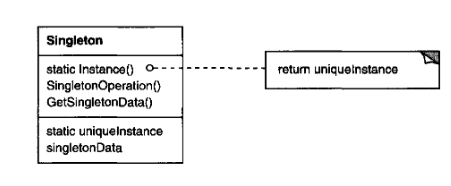
\includegraphics{figures/singleton.png}
    \caption{UML-Diagramm für Singleton}
    \label{fig:singleton}
\end{figure}

Die Abbildung~\ref{fig:singleton} zeigt den strukturellen Aufbau eines Singletons~\cite[S. 127]{gamma1994design}.
Dabei kann dieser nach Gamma et al. wie folgt beschrieben werden:

\begin{description}
    \item[Problem] \hfill \\
    \begin{itemize}
        \item Exakt eine Instanz der Klasse zur selben Zeit verfügbar; Zugreifbar zu Klienten durch bekannten Zugangspunkt
        \item Einzige Instanz erweiterbar durch Vererbung; Nutzbarkeit der Subklasse ohne Veränderung des Quellcodes auf Klientenseite
    \end{itemize}
    \item[Solution] \hfill
    \begin{itemize}
        \item   Zugriff auf Singleton-Instanz durch Instance-Operation
    \end{itemize}
    \item[Roles] \hfill \\
    \begin{description}
        \item[Singleton] \hfill \\
        \begin{itemize}
            \item Definiert eine Instance-Operation für Zugriff auf einzige Instanz
            \item Mögliche selbstsändige Instanziierung
        \end{itemize}
    \end{description}
    \item[Consequences]  \hfill 
    \begin{itemize}
        \item Kontrollierter Zugriff auf Instanz
        \item Mögliche Verfeinerung der Operationen und Repräsentation durch Vererbung
        \item Nachträgliche Änderung der Anzahl der Instanzen 
    \end{itemize}
\end{description}

\subsubsection{Factory Method}

\begin{figure}[h]
    \centering
    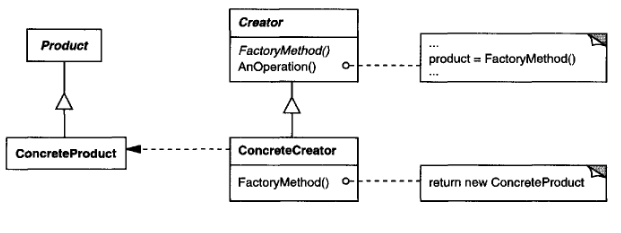
\includegraphics[scale=0.8]{figures/factory.png}
    \caption{UML-Diagramm für Factory Method}
    \label{fig:factory}
\end{figure}

Abbildung~\ref{fig:factory} beschreibt exemplarisch die Struktur einer Factory Method~\cite[S. 108]{gamma1994design}.
Diese wird nach Gamma et al. auf folgende Art und Weise beschrieben:

\begin{description}
    \item[Problem] \hfill 
    \begin{itemize}
        \item Eine Klasse kann die Klasse der Objekte, die es instantiiert, im Voraus nicht erahnen
        \item Eine Klasse verlangt, dass ihre Unterklassen die von ihr erstellten Objekte spezifizieren
        \item Klassen delegieren die Instantiierung von Objekten an Helferklassen
    \end{itemize}

    \item[Role] \hfill
    \begin{description}
        \item[Product] \hfill
        \begin{itemize}
            \item definiert die Schnittstelle der Objekte, die die Factory-Methode erzeugt
        \end{itemize}
        \item[ConcreteProduct] \hfill
        \begin{itemize}
            \item implementiert die Schnittstelle Product
        \end{itemize}
        \item[Creator] \hfill 
        \begin{itemize}
            \item deklariert die Factory-Methode, die ein Objekt vom Typ Product zurückgibt
            \item kann auch eine Standardimplementierung der Factory-Methode definieren, die die ein Standard ConcreteProduct-Objekt zurückgibt
            \item kann die Factory-Methode aufrufen, um ein Product-Objekt zu erzeugen
        \end{itemize}
        \item[ConcreteCreator] \hfill
        \begin{itemize}
            \item überschreibt die Factory-Methode, um eine Instanz eines ConcreteProduct zurückzugeben
        \end{itemize}
    \end{description}

    \item[Consequences] \hfill
    \begin{itemize}
        \item Eliminierung der Bindung an applikationsspezifische Klassen; Interaktion durch Product-Schnittstelle
        \item Flexibilität bei der Instanziierung von Objekten.
    \end{itemize}

\end{description}


%%TODO: Add concrete design patterns
\subsubsection{Structural Design Patterns}

Structural Design Patterns oder Strukturentwurfsmuster fokussieren sich darauf, wie einzelne Klassen und Objekte zusammengesetzt werden können, um größere Strukturen zu erzeugen\cite[S. 137]{gamma1994design}.
Entwurfsmuster dieser Kategorie sind vorteilhaft, wenn unabhängig voneinander entwickelte Klassen oder Objekte aus verschiedenen Bibliotheken oder Frameworks miteinander interagieren müssen.
Anstatt konkrete Implementierung und Schnittstellen zu nutzen, bedienen sich Structural Design Patterns der Komposition aus Objekten, um neue Funktionalitäten zur Verfügung zu stellen\cite[S. 137]{gamma1994design}.
Die dadurch gewonnene Flexibilität ermöglicht das Ändern der Zusammensetzung des Objektes dynamisch zu der Laufzeit, welches mit statischer Komposition durch Klassen nicht möglich ist.\cite[S. 137]{gamma1994design}.
Im Kontext dieser Arbeit werden folgende Entwurfsmuster aus der Kategorie der Structural Design Patterns betrachtet:

\subsubsection{Adapter}

\begin{figure}[h]
    \centering
    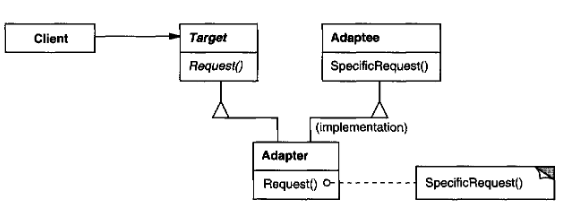
\includegraphics[scale=0.75]{figures/adapter.png}
    \caption{UML-Diagramm für Adapter}
    \label{fig:adapter}
\end{figure}

Abbildung~\ref{fig:adapter} zeigt die Struktur des Adapter-Entwurfsmusters. 
Dabei wird ein Adapter nach Gamma et al. wie gefolgt beschrieben~\cite[S. 141]{gamma1994design}:


.\begin{description}
    \item[Problem] \hfill
    \begin{itemize}
        \item Eine existierende Klasse soll genutzt werden; die Schnittstelle der Klasse stimmen mit der gebrauchten nicht überein
        \item Recyclebare Klasse, die mit unabhängigen Klassen kooperiert
    \end{itemize}
    \item[Roles] \hfill
    \begin{description}
        \item[Target] \hfill
        \begin{itemize}
            \item definiert domain-spezifische Schnittstelle für das Nutzen durch Clients
        \end{itemize}
        \item[Client] \hfill 
        \begin{itemize}
            \item kollaboriert mit Objekten, die Target-Schnittstelle implementieren
        \end{itemize}
        \item[Adaptee] \hfill 
        \begin{itemize}
            \item definiert ein bereits existierende Schnittstelle, worauf Adapter abgepasst wird
        \end{itemize}
        \item[Adapter] \hfill 
        \begin{itemize}
            \item adoptiert die Schnittstelle von Adaptee zu Target-Schnittstelle
        \end{itemize}
    \end{description}
    \item[Consequences] \hfill 
        \begin{itemize}
            \item Adoptierung von Adaptee zu Target-Schnittstelle durch konkrete Adapter-Klasse
            \item Adapter überschreibt Verhalten von Adaptee-Klasse, da Adapter Subklasse von Adaptee 
        \end{itemize}
\end{description}

\pagebreak

\subsubsection{Behavioral Design Patterns}

Behavioral Design Patterns oder Verhaltensentwurfsmuster konzentrieren sich auf Algorithmen und der Zuweisung von Verantwortlichkeiten zwischen Objekten\cite[S. 221]{gamma1994design}.
Dabei wird nicht nur Struktur der Entwurfsmuster betrachtet, sondern auch die Kommunikation und Interaktion der Objekte, die Teil des Entwurfsmusters sind. Charakteristisch für Design Patterns dieser Kategorie ist der Fokus auf Verknüpfung der einzelnen Teilobjekte des Entwurfsmusters,
anstatt des Kontrollflusses, welcher zur Laufzeit schwer nachvollziehbar sein kann~\cite[S. 221]{gamma1994design}.
Im Kontext dieser Arbeit werden folgende Entwurfsmuster aus der Kategorie der Behavioral Design Patterns betrachtet:

\subsubsection{Command}

\begin{figure}[h]
    \centering
    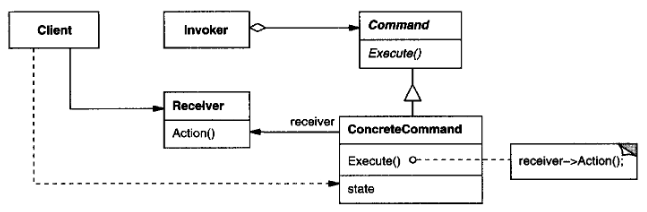
\includegraphics[scale=0.75]{figures/command.png}
    \caption{UML-Diagramm für Command}
    \label{fig:command}
\end{figure}

Abbildung~\ref{fig:command} zeigt die Struktur des Adapter-Entwurfsmusters. 
Dabei wird Command nach Gamma et al. wie gefolgt beschrieben~\cite[S. 236]{gamma1994design}:

\begin{description}
    \item[Problem] \hfill 
    \begin{itemize}
        \item Kapsulierung von Aktion durch parametrisierbare Objekte
        \item Spezifizierung, Abwarten und Ausführung von Aktionen zu verschiedenen Zeiten;
        \item Option für Undo; ausgeführte Aktion wird rückgängig gemacht
    \end{itemize}
    \item[Roles] \hfill
    \begin{description}
        \item[Command] \hfill
        \begin{itemize}
            \item deklariert eine Schnittstelle für das Ausführen von Operationen
        \end{itemize}
        \item[ConcreteCommand] \hfill
        \begin{itemize}
            \item definiert eine Bindung zwischen einem Receiver und einer Aktion
            \item implementiert Execute-Methode durch Ausführen des korrespondierenden Operationen auf Seite von Receiver
        \end{itemize}
        \item[Invoker] \hfill
        \begin{itemize}
            \item initialisiert die Ausführung eines Commands
        \end{itemize}
        \item[Receiver] \hfill
        \begin{itemize}
            \item Empfänger von Commands
            \item Wissen, wie empfangene Commands auszuführen sind  
        \end{itemize}
    \end{description}
    \item[Consequences] \hfill
    \begin{itemize}
        \item Entkoppelung zwischen Objekt, welches Operation initialisiert, und Objekt, das Operation durchführt
        \item Erweiterung von Manipulation von Verhalten von Command-Klassen durch Vererbung
        \item Zusammensetzung von Command-Klassen durch andere Command-Klassen
        \item Erleichtertes Hinzufügen von neuen Command-Klassen
    \end{itemize}
\end{description}

\subsubsection{Observer}

\begin{figure}[h]
    \centering
    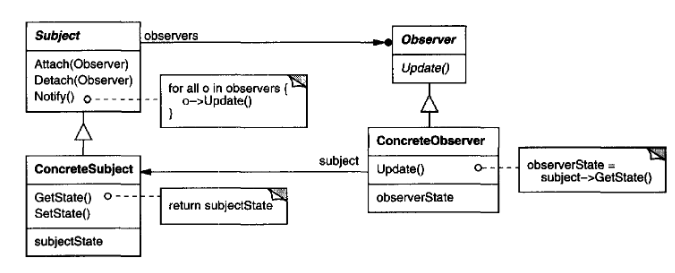
\includegraphics[scale=0.75]{figures/observer.png}
    \caption{UML-Diagramm für Observer}
    \label{fig:observer}
\end{figure}

Die Abbildung~\ref{fig:observer} zeigt den strukturellen Aufbau eines Observers~\cite[S. 293]{gamma1994design}.
Dabei kann dieser nach Gamma et al. wie folgt beschrieben werden:

\begin{description}
    \item[Problem] \hfill 
    \begin{itemize}
        \item Benachrichtigung von Objekten ohne Annahmen über diese
        \item Änderung in einem Objekt erfordert Änderungen in abhängigen Objekten; Kein Wissen wie abhängige Objekte auf Änderung reagieren
    \end{itemize}
    \item[Roles] \hfill
    \begin{description}
        \item[Subject] \hfill 
        \begin{itemize}
            \item Wissen über dessen Observer; beliebige Anzahl an Observern an einem Subject möglich
            \item Schnittstelle für das Hinzufügen und Entfernen von Observern
        \end{itemize}
        \item[Observer] \hfill 
        \begin{itemize}
            \item definiert Schnittstelle für das Reagieren von Änderungen am Subject seitens der abhängigen Objekte
        \end{itemize}
        \item[ConcreteSubject] \hfill 
        \begin{itemize}
            \item implementiert Subject-Schnittstelle
            \item beinhaltet relevanten Zustand von ConcreteObserver-Objekten
            \item Benachrichtigung von dessen Observer-Objekten bei Änderungen am relevanten Zustand
        \end{itemize}
        \item[ConcreteObserver] \hfill 
        \begin{itemize}
            \item hält Referenz zu ConcreteSubject-Objekt
            \item Speichert selbst Zustand; konsistent zu dem von Subject
            \item implementiert Observer-Schnittstelle für das Synchronisieren der Zustände  
        \end{itemize}
    \end{description}
    \item[Consequences]:
    \begin{itemize}
        \item Abstrakte Koppelung zwischen Observer und Subject; Keine Annahmen von Subject über Observer außer Observer-Schnittstelle
        \item Broadcast an Observer; Benachrichtigung aller registrierten Observer
        \item Einspielen von unerwarteten Benachrichtigung 
    \end{itemize}
\end{description}
\section{Herausforderungen und Probleme bei der Erkennung von Design Patterns}

In diesem Abschnitt der Arbeit werden mögliche Herausforderungen diskutiert, die bei dem Entwerfen des Prozesses für die Erkennung von Entwurfsmustern auftreten können. 

\subsection*{Variabilität der Implementierung}

Design Patterns stellen in der Software-Entwicklung bewährte Lösungsmuster für bereits begegnete Herausforderung dar. Aufgrund der abstrakten und wiederverwendbaren Natur der Entwurfsmuster,
muss für diese eine konkrete Implementierung definiert werden, die von dem Einsatzfall, Kontext und anderen Faktoren wie verwendeter Programmiersprache, Bibliotheken und Erfahrungsstand des Software-Entwicklers.
Dadruch, dass jedes Entwurfsmuster einen konzeptionellen Rahmen darstellt und jede Implementierung von nicht statischer Außenfaktoren beeinflusst wird, resultiert dies in einem breiten Spektrum an Implementierungen für ein gegebenes Entwurfsmuster.
Aus diesem Grund ist eine Definition einer starren Definition eines Design Patterns, was als Startpunkt und Referenz für die Erkennung des jeweiligen Entwurfsmusters dienen könnte, nicht möglich. 
Deshalb ist eine definitive Antwort auf die Frage, ob eine betrachte Mikroarchitektur eine Instanz eines Entwurfsmusters, nicht beantwortbar, weshalb die Antwort von automatisierten Prozessen von Design Patterns eher mit einem Wert besteht,
welches die Ähnlichkeit zu einem Design Pattern beschreibt. Um einen zufriedenstellenden Wert für diese Frage zu liefern, bedarf es eines bereiten Spektrums an Implementierungsvariationen als Referenz für die Erkennung.

\subsection*{Steigende Komplexität von Software-Systemen}

Die steigende Komplexität von Software-Systemen stellt eine erhebliche Herausforderung bei der Erkennung von Entwurfsmustern in Entwurfsmustern dar.
Dies ist besonders bei langjährigen Software-Projekten der Fall, an denen über die Zeit konstante Änderungen wegen Wartung und neuen bzw. geänderten Anforderungen unterliegen.
Diese Art von Software-Projekten tendieren dazu, dass mit der Zeit deren Komplexität zunimmt~\cite[S. 7]{Suh-2010}. 
Bei kleineren Software-Projekten mit geringem Umfang und Komplexität sind Entwurfsmuster leichter zu erkennen und zu implementieren.
Dahingegen bei langjährigen Software-Projekten steigt mit wachsender Gesamtkomplexität die Komplexität der angewendeten Entwurfsmuster in deren Quellcode, wodurch die Identifizierung dieser proportional mitsteigt.
Entwurfsmuster werden durch diese Entwicklung weiter modifiziert und angepasst, womit diese von der ursprünglichen leichter zu identifizierbaren Iterationen weiter abweichen. 
Deshalb beinhaltet die Erkennung von Entwurfsmustern nicht nur auf die momentane Iteration, sondern auch die Erfassung derer historischen Evolution und die Entwicklung dieser innerhalb der Codebasis.

\newpage

\subsection*{Iterative Evolution des Quellcodes}

Damit ein Software-System seine Anforderungen im Verlauf dessen Lebenszyklus in einer zufriedenstellenden Art und Weise erfüllen kann, muss dieses adaptieren, um diesen Anforderungen gerecht zu werden~\cite[S. 108]{10.1007/BFb0017737}.
Dies hat zu Folge, dass dessen Quellcode iterativen Änderungen unterliegt. Ursprüngliche Implementierungen in der Codebasis werden analysiert und es wird überprüft, ob diese ihre Aufgaben zufriedenstellend erfüllen oder nicht.
Falls nicht, werden diese so modifiziert, sodass diese Anforderungen auf erwartete Art und Weise erfüllt werden können. Implementierungen von angewandten Design Patterns als Teil des Quellcodes unterliegen ebenfalls dieser Analyse.
Diese werden als Teil des Analyseprozesses genauer betrachtet und werden nach Bedarf modifiziert und angepasst. Diese Entwicklung führt wie das im vorherigen Abschnitt diskutierten Fall, dass Entwurfsmuster von ihrer ursprünglichen leichter zu identifizierbaren
Iteration weiter abweichen und die Erkennung von Entwurfsmustern nicht nur die momentane Implementierung, sondern auch die historische Entwicklung berücksichtigen werden muss. In automatisierten Prozess der Erkennung von Entwurfsmustern kann dieser Aspekt nur bedingt berücksichtigt,
weil das Einschließen der Historie der betrachtenden Implementierung und dessen Kontext in der Codebasis nicht pauschal und in einer allgemeinen Ansicht betrachtet werden kann. 

\subsection*{Mangel an expliziter Dokumentation}

Das Erstellen und Warten von Dokumentation für Software-Systeme ist eine Tätigkeit, die von Software-Entwicklern als wichtig eingestuft wird, jedoch in diese Tätigkeit relativ wenig Zeit investiert wird~\cite[S, 162]{zhi2015cost}.
Dies ist die Folge der Dominanz des agilen Software-Entwicklungsprozesses, in dieser die Verwendung von Zeit und Ressourcen für die Dokumentation eher als Verschwendung betrachtet wird, da diese keinen direkten Mehrwert für die Auslieferung des Software-Produktes an den Endkunden liefert~\cite[S. 159]{zhi2015cost}.
Das dies das Software-System komplett betrifft, sind Design Patterns in dessen Codebasis ebenfalls betroffen. Diese werden meist nicht direkt gekennzeichnet. 
Zwar kann durch Nomenklatur und Kontrollfluss indirekt Rückschlüsse auf die potenziellen Entwurfsmuster abgeleitet werden, jedoch erfordert dies konkretes Fachwissen und Erfahrungen, die nicht von jedem Software-Entwickler erfüllt werden kann.
Bei automatisierten Prozessen für die Erkennung von Entwurfsmustern kann diese berücksichtigt werden, sollte aber nicht als alleiniger Faktor bei dem Identifikationsprozess dienen.\\

Aufgrund der Variation an Implementierungsmöglichkeiten, Änderungen im Quellcode und Mangel an Dokumentation ist die manuelle Identifikation von Entwurfsmustern in Quellcode ein Prozess dar,
in der einen gewissen Grad an Mitdenken erfordert. Im nächsten Abschnitt der Arbeit werden bereits entwickelte Verfahren betrachtet, die das Mitdenken bis zu einem gewissen Grad automatisieren und dieses als Teil des Prozesses mitinludieren.





\section{Alternative Ansätze}
\section{Angewendete Ansätze mit Maschine Learning}
\section{Verfügbare Datensätze}\label{dataset}
Um ein Machine Learning Modell zu trainieren, benötigt es einen Datensatz mit passenden gekennzeichneten Klassen.
In der Erkennung von Entwurfsmustern existiert zu dem Zeitpunkt der Verfassung dieser Arbeit keine standardmäßiger oder weit akzeptierter Datensatz.
Jedoch existieren Versuche, solch einen Datensatz zu etablieren. Im Folgenden wird eine Auswahl an möglichen existierenden Datensätzen aufgelistet~\cite[S. 104 - 105]{phdthesis}:

\begin{description}
    \item Pattern-like Micro-Architecture Repository (P-MArt): Dieser Datensatz ist der einzige der hier aufgelisteten, welcher Peer-Reviews unterzogen wurde. Zwar bestehen die Autoren nicht darauf, dass alle möglichen Instanzen von Entwurfsmustern in den Software-Systemen identifiziert wurden, haben aber Zuversicht, dass die Mehrheit der Instanzen durch mehrfache Analysen durch mehrere Teams erkannt wurde. 
    \item DEsign pattern Evaluation BEnchmark Environment (DEEBEE): Dieser Datensatz beinhaltet Resultate aus automatischer und einer manuellen Analyse von fünf Software-Systemen auf Entwurfsmustern.
    \item Design Pattern Benchmark (DPD): DPD beinhaltet die Ergebnisse von Software-Systemen durch mehrere Software-Werkzeuge. Zudem sind die Daten des Datensatzes durch eine Webseite verfügbar, in der nach Instanzen von Entwurfsmustern in Software-Systemen gesucht werden kann. Zusätzlich können auf dieser Webseite Ergebnisse evaluiert und durch öffentlich zugängliche Abstimmung einer Instanz das passende Design Pattern zugeordnet werden.
    \item PattErn Repository and Components Extracted from OpeN Source software (PERCERONS): PERCERONS ist das derzeit von dem Umfang her der größte verfügbare Datensatz mit über 537 analysierten Software-Systemen. Die Ergebnisse wurden durch das Kombinieren der Resultate zweier Software-ErgebnisWerkezeuge ermittelt.
    \item Software Engineering Research Center benchmark (SERC): SERC wurde konstruiert, um als Vergleichsmaßstab für ein Software-Werkzeug zu dienen, welches von den gleichen Autoren stammte. Dabei werden die Ergebnisse von mehreren anderen Werkzeugen mit den Ergebnissen ihres eigenes kombiniert.
\end{description}

Die Problematik bei der Ermittelung eines geeigneten Datensatzes besteht darin, dass der Umfang der analysierten Software-Systeme sich in Grenzen hält und meist eher als Maßstab für die Leistung der selbst entwickelten Methode verwendet wird, wodurch Bias zu der eignen Methode nicht ausgeschlossen werden kann.
Zudem sind die hier aufgeführten Datensätze bis auf einige Ausnahmen durch die Kombination von mehreren Software-Werkzeugen entstanden. Durch solch ein Verfahren ist zwar die Analyse von mehreren Software-Systemen in einer relativ kurzen Zeitspanne möglich, jedoch wäre eine manuelle Verifizierung der Ergebnisse aufgrund von hohen Zeit- und Leistungsaufwands schwer umsetzbar.
Dahingegen wäre das ideale Vorgehen, das solch ein Datensatz durch manuelles Identifizieren von Entwurfsmustern in Quellcode durch die Analyse von mehreren Software-Systemen durch ein Experten-Team erstellt wird. Jedoch ist solch ein Verfahren zeitaufwendig und erfordert ein tiefes Verständnis des jeweiligen Software-Systems, welches durch mangelnde oder obsolete Dokumentation eine Hürde darstellt.
Die nächst bestmögliche Alternative dazu ist die Option des Crowdsourcings wie in DPD. Das Problem ist hier, dass die Qualifikation der Personen, die Instanzen von Entwurfsmustern identifizieren und über die korrekte Zuweisung abstimmen, nicht garantiert sind. Zudem erfordert dies ein Publikum mit der Bereitschaft, dies zu tun, welches auch nicht garantiert werden kann.
Bei dem im Kontext dieser Arbeit vorgestellten Verfahren für die Ermittelung von Entwurfsmustern wird meist ein Datensatz im kleinen Umfang erstellt. Auf Anfrage. um Zugang zu einigen Datensätzen zu erhalten, gibt es zu dem Zeitpunkt zur Verfassung dieser Arbeit keine Antwort seitens der Autoren. Zudem sind die Webseiten, worüber auf die Datensätze zugegriffen werden kann, nicht mehr verfügbar und der Zugang über eine Archivierungsdienstleistung wie der Wayback Maschine war ebenfalls nicht möglich. 
Aus den hier aufgelisteten Gründen wird im Zuge dieser Arbeit der P-MArt Datensatz verwendet und somit die Untersuchungsfrage~\ref{RQ2} zu beantworten. Dieser ist zum Zeitpunkt des Verfassens dieser Arbeit zugänglich und ist der Einzige, der Peer-Reviews unterzogen wurde. In der Sektion der Implementierung wird dieser genauer betrachtet.
\section{Feature Engineering}
\section{Betrachte Multiclass-Klasszifizierer}
\section{Metriken für Klasszifizierer}
\section{Angewendete Technologien, Frameworks und Bibliotheken}

\chapter{Methodologie}
\section{Verfügbare Datensätze}\label{dataset}
Um ein Machine Learning Modell zu trainieren, benötigt es einen Datensatz mit passenden gekennzeichneten Klassen.
In der Erkennung von Entwurfsmustern existiert zu dem Zeitpunkt der Verfassung dieser Arbeit keine standardmäßiger oder weit akzeptierter Datensatz.
Jedoch existieren Versuche, solch einen Datensatz zu etablieren. Im Folgenden wird eine Auswahl an möglichen existierenden Datensätzen aufgelistet~\cite[S. 104 - 105]{phdthesis}:

\begin{description}
    \item Pattern-like Micro-Architecture Repository (P-MArt): Dieser Datensatz ist der einzige der hier aufgelisteten, welcher Peer-Reviews unterzogen wurde. Zwar bestehen die Autoren nicht darauf, dass alle möglichen Instanzen von Entwurfsmustern in den Software-Systemen identifiziert wurden, haben aber Zuversicht, dass die Mehrheit der Instanzen durch mehrfache Analysen durch mehrere Teams erkannt wurde. 
    \item DEsign pattern Evaluation BEnchmark Environment (DEEBEE): Dieser Datensatz beinhaltet Resultate aus automatischer und einer manuellen Analyse von fünf Software-Systemen auf Entwurfsmustern.
    \item Design Pattern Benchmark (DPD): DPD beinhaltet die Ergebnisse von Software-Systemen durch mehrere Software-Werkzeuge. Zudem sind die Daten des Datensatzes durch eine Webseite verfügbar, in der nach Instanzen von Entwurfsmustern in Software-Systemen gesucht werden kann. Zusätzlich können auf dieser Webseite Ergebnisse evaluiert und durch öffentlich zugängliche Abstimmung einer Instanz das passende Design Pattern zugeordnet werden.
    \item PattErn Repository and Components Extracted from OpeN Source software (PERCERONS): PERCERONS ist das derzeit von dem Umfang her der größte verfügbare Datensatz mit über 537 analysierten Software-Systemen. Die Ergebnisse wurden durch das Kombinieren der Resultate zweier Software-ErgebnisWerkezeuge ermittelt.
    \item Software Engineering Research Center benchmark (SERC): SERC wurde konstruiert, um als Vergleichsmaßstab für ein Software-Werkzeug zu dienen, welches von den gleichen Autoren stammte. Dabei werden die Ergebnisse von mehreren anderen Werkzeugen mit den Ergebnissen ihres eigenes kombiniert.
\end{description}

Die Problematik bei der Ermittelung eines geeigneten Datensatzes besteht darin, dass der Umfang der analysierten Software-Systeme sich in Grenzen hält und meist eher als Maßstab für die Leistung der selbst entwickelten Methode verwendet wird, wodurch Bias zu der eignen Methode nicht ausgeschlossen werden kann.
Zudem sind die hier aufgeführten Datensätze bis auf einige Ausnahmen durch die Kombination von mehreren Software-Werkzeugen entstanden. Durch solch ein Verfahren ist zwar die Analyse von mehreren Software-Systemen in einer relativ kurzen Zeitspanne möglich, jedoch wäre eine manuelle Verifizierung der Ergebnisse aufgrund von hohen Zeit- und Leistungsaufwands schwer umsetzbar.
Dahingegen wäre das ideale Vorgehen, das solch ein Datensatz durch manuelles Identifizieren von Entwurfsmustern in Quellcode durch die Analyse von mehreren Software-Systemen durch ein Experten-Team erstellt wird. Jedoch ist solch ein Verfahren zeitaufwendig und erfordert ein tiefes Verständnis des jeweiligen Software-Systems, welches durch mangelnde oder obsolete Dokumentation eine Hürde darstellt.
Die nächst bestmögliche Alternative dazu ist die Option des Crowdsourcings wie in DPD. Das Problem ist hier, dass die Qualifikation der Personen, die Instanzen von Entwurfsmustern identifizieren und über die korrekte Zuweisung abstimmen, nicht garantiert sind. Zudem erfordert dies ein Publikum mit der Bereitschaft, dies zu tun, welches auch nicht garantiert werden kann.
Bei dem im Kontext dieser Arbeit vorgestellten Verfahren für die Ermittelung von Entwurfsmustern wird meist ein Datensatz im kleinen Umfang erstellt. Auf Anfrage. um Zugang zu einigen Datensätzen zu erhalten, gibt es zu dem Zeitpunkt zur Verfassung dieser Arbeit keine Antwort seitens der Autoren. Zudem sind die Webseiten, worüber auf die Datensätze zugegriffen werden kann, nicht mehr verfügbar und der Zugang über eine Archivierungsdienstleistung wie der Wayback Maschine war ebenfalls nicht möglich. 
Aus den hier aufgelisteten Gründen wird im Zuge dieser Arbeit der P-MArt Datensatz verwendet und somit die Untersuchungsfrage~\ref{RQ2} zu beantworten. Dieser ist zum Zeitpunkt des Verfassens dieser Arbeit zugänglich und ist der Einzige, der Peer-Reviews unterzogen wurde. In der Sektion der Implementierung wird dieser genauer betrachtet.
\section{Feature Engineering}
\section{Angewendete Multiclass-Klasszifizierer}
\section{Evaluation des trainierten Models}
\section{Modellauswahl, Training und Validierung}
Nach dem Bestimmen eines passenden Datensatzes und zu extrahierenden Features wird ein Klassifizierer trainiert, welcher mit einem Wahrscheinlichkeitswert angibt, welche Rolle am ehesten der Quellcodeentität zugeordnet werden kann.
Dazu wird in dieser Sektion erläutert, welche Modelle betrachtet werden und wie diese trainiert und evaluiert werden können. 


\subsection*{Auswahl der Klassifizierer}
Im Zuge dieser Arbeit werden in der Sektion \ref{classifiers} erläuterten Klassifizierer als die bevorzugten Modelle hergenommen. Diese Auswahl der Modelle ist auf unterschiedliche Gründe zurückzuführen.
Klassifizierer können je nach Art und Weise, wie sie innerlich funktionieren, in Kategorien untergliedert werden. Dabei dienen die Modelle aus Sektion \ref{classifiers} als Repräsentanten ihrer Kategorie, sodass ein Spektrum von unterschiedlich funktionierenden Modellen getestet werden kann.
Ohne das Testen des jeweiligen Models ist dessen Leistung für das in dieser Arbeit genutzten Datensatzes nicht vorherzusagen. Zudem können Implementierungen der jeweiligen Modelle in verschiedenen Programmiersprachen für verschiedene Plattformen vorgefunden werden.
Dies ermöglicht die Nutzung in Programmiersprachen wie Python oder R, welche für Machine Learning bevorzugt werden. Das Software-Framework, welches die Implementierungen für die Modelle zur Verfügung stellt und im Kontext dieser Arbeit angewendez wird, wird im weiteren Verlauf der Arbeit genauer erläutert.
Der größte Vorteil dieser Klassifizierer ist deren Simplizität und damit resultierende Effizienz in Zeit- und Speicherkomplexität. Da die Klassifizierer im weiteren Verlauf der Methode durch den Einsatz von Hyperparameter-Tuning iterativ optimiert werden, ist dies von besonderer Bedeutung.
Deshalb werden Modelle mit komplexerer Architektur aufgrund des Mangels verfügbarer Rechenressourcen zu Zeitpunkt des Verfassens der Arbeit nicht weiter betrachtet. 
Die Auswahl der Klassifizierer aus Sektion~\ref{classifiers} beantwortet die Untersuchungsfrage~\ref{RQ5}


\subsection*{Training der Modelle}
In dieser Arbeit wird das Trainieren der Modelle mit dem Hyperparameter-Tuning aus Sektion~\ref{hyper_params} gekoppelt. Zuerst wird der Datensatz in ein Trainings- und Validationsdatensatz aufgeteilt. Danach wird für jedes Modell ein Suchraum für die Hyperparameter-Werte, Anzahl der Trainingsiterationen und die Metrik bestimmt, wonach die Leistung des Klassifizierers
beurteilt wird. In jeder Iteration wird zufällig eines der hier vorgestellten Klassifizierer mit einer vorher bestimmten Hyperparameter-Konfiguration instanziiert, mit dem Trainingsdatensatz trainiert und durch Einsatz des Validationsdatensatzes der Wert der Leistungsmetrik bestimmt. Die Hyperparameter-Konfiguration der Instanz mit der besten Leistung aus allen Iterationen wird im weiteren Verlauf der Arbeit verwendet.

\subsection*{Validierung des Modells}
Dadruch, dass der Datensatz für das Training aufgeteilt wird, wird die beste Hyperparameter-Konfiguration eines der hier vorgestellten Klassifizierer durch Kreuzvalidierung zusätzlich validiert. 
Dabei wird der gesamte verfügbare Validationsdatensatz verwendet. Die Evaluierung der Leistung der Klassifikationskapazität erfolgt mit der gleichen Metrik wie in der Trainingsphase. Es bestünde die Option, dass man die Kreuzvalidierung direkt in die Trainingsphase integriert. 
Jedoch ist dabei zu beachten, dass die Kreuzvalidierung selbst iterativ agiert und dies in jeder Iteration des Hyperparameter-Tunings durchgeführt wird. Dies erhöht die Laufzeit der Trainingsphase signifikant.
\section{Evaluation der Methodologie}

\chapter{Zukünftige Aussichten}
\section{Zukünftige Aussichten}

Die fortschrittlichen Entwicklungen im Bereich des maschinellen Lernens (ML) und speziell der Large Language Models (LLMs) eröffnen neue Perspektiven für die automatisierte Erkennung von Design Patterns in Quellcode. In dieses Feld wurden zum Zeitpunkt der Verfassen der Arbeit Fortschritte getätigt, da LLMs das Potenzial geben, die Effizienz und Genauigkeit bei der Identifizierung von Design Patterns erheblich zu verbessern. Im Folgenden werden die zukünftigen Aussichten dieser Technologie beleuchtet.

\begin{enumerate}
    \item \textbf{Erweiterte Erkennungskapazitäten}: Mit der zunehmenden Verfeinerung von LLMs ist zu erwarten, dass ihre Fähigkeit, komplexe Muster und Abstraktionen im Quellcode zu erkennen, deutlich zunimmt. Diese Modelle können aus einer umfangreichen Datenmenge lernen und somit eine breite Palette von Design Patterns identifizieren, die in verschiedenen Programmiersprachen und -stilen zum Einsatz kommen. Die Flexibilität von LLMs ermöglicht es ihnen, auch seltene oder weniger dokumentierte Patterns zu erkennen, die herkömmliche Methoden möglicherweise übersehen.
    \item \textbf{Verbesserung der Präzision und Reduzierung von Fehlalarmen}: Durch das Training mit großen Datensätzen können LLMs nicht nur eine Vielzahl von Patterns erkennen, sondern auch den Kontext, in dem diese Patterns verwendet werden, besser verstehen. Dies führt zu einer höheren Präzision bei der Erkennung und einer signifikanten Reduzierung von Fehlalarmen. Die Fähigkeit, den Kontext zu berücksichtigen, ist besonders wichtig, da viele Design Patterns nur in bestimmten Situationen angemessen sind. LLMs können feine Unterschiede im Code erfassen, die darauf hinweisen, ob ein bestimmtes Pattern tatsächlich beabsichtigt ist oder nicht.
    \item \textbf{Automatisierte Verbesserungsvorschläge und Refactoring}: Zukünftige Entwicklungen könnten LLMs befähigen, nicht nur existierende Patterns zu erkennen, sondern auch Verbesserungsvorschläge zu machen. Basierend auf der erkannten Implementierung eines Design Patterns könnten diese Modelle Empfehlungen für ein effizienteres oder klareres Pattern geben, das in den aktuellen Code eingeführt werden kann. Darüber hinaus ist das Potenzial für automatisiertes Refactoring beträchtlich, wobei LLMs Vorschläge für Code-Umstrukturierungen machen können, um Design Principles wie SOLID besser einzuhalten.
    \item \textbf{Interaktive Entwicklungsumgebungen}: Die Integration von LLMs in Entwicklungsumgebungen und IDEs (Integrated Development Environments) könnte zu einer interaktiveren und unterstützenden Codierungserfahrung führen. Entwickler könnten in Echtzeit Feedback zu den von ihnen verwendeten Design Patterns erhalten, einschließlich Hinweisen zur Anwendung und möglichen Optimierungen. Diese Art der direkten Integration fördert ein tieferes Verständnis für Design Patterns und unterstützt Entwickler dabei, best practices effektiver in ihren Code zu integrieren.
\end{enumerate}




\appendix
\chapter{Zusätzliche Tabellen für die Datenanalyse von P-MArt}


\begin{table}[H]
    \centering
    \begin{tabular}{|c|c|}
        \hline
        Rolle & Aufkommen in Datensatz\\
        \hline
        abstractclass & 7\\abstractfactory & 2\\abstraction & 1\\abstractproduct & 3\\adaptee & 17\\adapter & 29\\aggregate & 5\\builder & 1\\caretaker & 5\\client & 64\\colleague & 2\\command & 6\\component & 7\\composite & 11\\concreatecolleague & 4\\concreteaggregate & 6\\concretebuilder & 14\\concreteclass & 51\\concretecommand & 50\\concretecomponent & 55\\concretecreator & 13\\concretedecorator & 6\\concreteelement & 102\\concretefactory & 8\\concreteimplementor & 4\\concreteiterator & 8\\concretemediator & 2\\concreteobserver & 28\\concreteproduct & 38\\concreteprototype & 3\\concretestate & 21\\concretestrategy & 68\\concretesubject & 59\\concretevisitor & 29\\context & 24\\creator & 6\\decorator & 1\\director & 4\\element & 5\\facade & 1\\implementor & 1\\invoker & 29\\iterator & 4\\leaf & 92\\mediator & 2\\memento & 8\\nullobject & 1\\objectstructure & 4\\observer & 9\\originator & 8\\product & 46\\prototype & 1\\proxy & 5\\realsubject & 5\\receiver & 12\\refinedabstraction & 3\\singleton & 15\\state & 5\\strategy & 6\\subject & 9\\subsystemclass & 10\\target & 10\\visitor & 5\\
        \hline
    \end{tabular}
    \caption{tabellarische Darstellung der Rollenverteilung in P-MArt}
\end{table}

%%% Local Variables: 
%%% mode: latex
%%% TeX-master: "thesis.tex"
%%% End: 


\cleardoublepage

\bibliographystyle{natger}
\bibliography{thesis}

\cleardoublepage


\footnotesize
\printindex


\end{document}
